% This work is licensed under the Creative Commons
% Attribution-NonCommercial-ShareAlike 4.0 International License. To view a copy
% of this license, visit http://creativecommons.org/licenses/by-nc-sa/4.0/ or
% send a letter to Creative Commons, PO Box 1866, Mountain View, CA 94042, USA.

\section{Elemente der Linearen Algebra}
Ziel: Bereitstellung einiger Hilfsmittel aus der linearen Algebra.
Literatur:
\begin{enumerate}[label=(\arabic*)]
	\item G. Fischer (1997) \emph{Lineare Algebra} \cite{fischerLinAlg}
	\item M. Koecher (1997) \emph{Lineare Algebra und analytische Geometrie} \cite{koecher2013lineare}
\end{enumerate}

Im gesamten Abschnitt ist
\begin{align*}
	\R^n:=\set{\begin{pmatrix}
		x_1\\
		\vdots\\
		x_n
	\end{pmatrix}
	:x_i\in\R\quad\forall 1\leq i\leq n}\qquad\forall n\in\N
\end{align*}
der gewöhnliche \define{euklidische Raum} versehen mit dem kanonischen Skalarprodukt
\begin{align*}
	\scaProd{x}{y}:=\sum\limits_{i=1}^n x_i\mal y_i\qquad\forall x,y\in\R^n
\end{align*}
und zugehöriger \define{euklidische Norm}
\begin{align*}
	\norm{x}:=\sqrt{\scaProd{x}{x}}
	=\sqrt{\sum\limits_{i=1}^n x_i^2}
	\qquad\forall x\in\R
\end{align*}

\setcounter{satz}{-1}
\begin{definition}\label{def2.0}\
	\begin{enumerate}[label=(\arabic*)]
		\item $x,y\in\R^n$ heißen \define{orthogonal}, in Zeichen
		\index{orthogonal}
		\begin{align*}
			x\perp y:\iff\scaProd{x}{y}=0
		\end{align*}
		\item Sei $U\subseteq\R^n$ und $x\in\R^n$. Dann setze
		\begin{align*}
			x\perp U:\iff\forall u\in U: x\perp u
		\end{align*}
		\item Das \define{orthogonale Komplement} von $U\subseteq\R^n$ ist
		\index{orthogonales Komplement}
		\begin{align*}
			U^\perp:=\set{x\in\R^n:x\perp U}
		\end{align*}
	\end{enumerate}
\end{definition}

\begin{satz}\label{satz2.1}\
	\begin{enumerate}[label=(\arabic*)]
		\item $\begin{aligned}
			x\perp y\implies \norm{x+y}^2=\norm{x}^2+\norm{y}^2
		\end{aligned}$ (Pythagoras)\label{item:satz2.1(1)}
		\index{Pythagoras}
		\item $U^\perp$ ist Untervektorraum (UVR / UR) von $\R^n$\label{item:satz2.1(2)}
		\item Falls $U\subseteq\R^n$ UVR von $\R^n$ ist, gilt:\label{item:satz2.1(3)}
		\begin{enumerate}[label=(\roman*)]
			\item $\begin{aligned}\label{item:satz2.1(3i)}
				U\cap U^\perp=\set{0}
			\end{aligned}$
			\item $\begin{aligned}
				\big(U^\perp)^\perp=U\label{item:satz2.1(3ii)}
			\end{aligned}$
		\end{enumerate}
	\end{enumerate}
\end{satz}

\begin{proof}
	\betone{Zeige \ref{item:satz2.1(1)}:}
	\begin{align*}
		\norm{x+y}^2
		&=\scaProd{x+y}{x+y}
		=\underbrace{\scaProd{x}{x}}_{=\norm{x}^2}+2\mal\underbrace{\scaProd{x}{y}}_{=0}+\underbrace{\scaProd{y}{y}}_{=\norm{y}^2}
	\end{align*}
	\betone{Zeige \ref{item:satz2.1(2)}:} Seien $x,y\in U^\perp$ und seien $\alpha,\beta\in\R$
	\begin{align*}
		\scaProd{\alpha\mal x+\beta\mal y}{u}
		\overset{\Lin}&{=}
		\alpha\mal\underbrace{\scaProd{x}{u}}_{=0}+\beta\mal\underbrace{\scaProd{y}{u}}_{=0}\qquad\forall u\in U\\
		&\implies\alpha\mal x+\beta\mal y\in U^\perp
	\end{align*}
	\betone{Zu \ref{item:satz2.1(3)} zeige \ref{item:satz2.1(3i)}:}
	Da $U$ und $U^\perp$ Vektorräume sind, gilt $0\in U,U^\perp$ und somit $U\cap U^\perp\supseteq\set{0}$.
	\begin{align*}
		x\in U\cap U^\perp\implies\scaProd{x}{x}=0
		\implies\norm{x}=0
		\implies x=0
	\end{align*}
	\betone{Zu \ref{item:satz2.1(3)} zeige \ref{item:satz2.1(3ii)}:} 
	Zeige "$\supseteq$":
	Sei $x\in U$ und $y\in U^\perp$. Zeige
	\begin{align}\label{eq:ProofSatz2.1Stern}\tag{$*$}
		\scaProd{x}{y}=0
	\end{align}
	Da $y\in U^\perp$, gilt $\scaProd{y}{u}=0$ für alle $u\in U$, also insbesondere für $u=x\in U$.
	Somit folgt \eqref{eq:ProofSatz2.1Stern}.\\
	Für Teil "$\subseteq$" siehe Koecher \cite{koecher2013lineare}, Seite 160.
\end{proof}

\begin{satz}\label{satz2.2}
	Seien $U,V\subseteq\R^n$ UVR des $\R^n$ und 
	\begin{align*}
		U+V:=\set{u+v:u\in U,v\in V}\subseteq\R^n
	\end{align*}
	die \define{Summe} von $U$ und $V$.
	Dann ist $U+V$ wieder ein UVR von $\R^n$.
	Falls $U\cap V=\set{0}$, so schreibt man
	\begin{align*}
		U\oplus V:=U+V
	\end{align*}
	für die \define{direkte Summe} von $U$ und $V$.
	\index{direkte Summe}
	Es gilt:
	\begin{align*}
		x\in U\oplus V\implies\exists! u\in U,\exists! v\in V: x=u+v
	\end{align*}
	Wichtig ist hierbei, dass $u\in U$, $v\in V$ \betone{eindeutig} bestimmt sind.
\end{satz}

\begin{proof}
	Dass $U+V$ bzw. $U\oplus V$ ein  UVR ist, ist klar.\\
	Sei $x\in U\oplus V$ und angenommen $x=u+v=\tilde{u}+\tilde{v}$ mit $u,\tilde{u}\in U$ und $v,\tilde{v}\in V$.
	Dann folgt:
	\begin{align*}
		u+v=\tilde{u}+\tilde{v}
		\implies
		\underbrace{u-\hat{u}}_{\in U}=\underbrace{\tilde{v}-v}_{\in V}\in U\cap V
		\overset{\Vor}{=}\set{0}\\
		\implies u=\tilde{u}\und\tilde{v}=v
	\end{align*}
\end{proof}

\begin{satz}\label{satz2.3}
	Für jeden UVR $U\subseteq\R^n$ des $\R^n$ gilt:
	\begin{align*}
		\R^n=U\oplus U^\perp
	\end{align*}
\end{satz}

\begin{proof}
	Siehe Fischer \cite{fischerLinAlg}, Seite 283.
\end{proof}

\begin{definition}\label{def2.4}
	Sei $U\subseteq\R^n$ UVR des $\R^n$.	
	Gemäß Satz \ref{satz2.2} und Satz \ref{satz2.3} existiert für jedes $x\in\R^n$ genau ein Paar 
	$(u,v)\in U\times U^\perp$ mit $x=u+v$.
	Die Abbildung
	\begin{align*}
		P=P_U\colon \R^n\to U\subseteq\R^n,\qquad P(x):= u
	\end{align*}
	ist wegen Satz \ref{satz2.2} und Satz \ref{satz2.3} wohldefiniert.
	Weitere Bezeichnung:
	$P=P_U$ heißt \define{orthogonale Projektion auf $U$}.
	\index{orthogonale Projektion}
	Analog: $P_{U^\perp}(x):=v$.
\end{definition}

\begin{satz}\label{satz2.5}\
	\begin{enumerate}[label=(\arabic*)]
		\item $P=P_U$ ist linear \label{item:satz2.5(1)}
		\item $\begin{aligned}
			P(u)=u\qquad\forall u\in U \label{item:satz2.5(2)}
		\end{aligned}$
	\end{enumerate}
\end{satz}

\begin{proof}
	\betone{Zeige \ref{item:satz2.5(1)}:}
	Seien $x_1,x_2\in\R^n$. Dann:
	\begin{align*}
		x_i&=u_i+v_i,\qquad\exists u_i\in U,~v_i\in U^\perp\\
		i\in\set{1,2}\implies
		x_1+x_2&=\big(u_1+v_1\big)+\big(u_2+v_2\big)
		\overset{\text{Kommu+Asso}}{=}\big(\underbrace{u_1+u_2}_{\in U}\big)+\big(\underbrace{v_1+v_2}_{\in U^\perp}\big)\\
		\implies P(x_1+x_2)&=P\klammern[\Big]{\big(\underbrace{u_1+u_2}_{\in U}\big)+\big(v_1+v_2\big)}
		\overset{\Def}{=}u_1+u_2
		\overset{\Def}{=}P(x_1)+P(x_2)\\
		&\implies P\text{ ist additiv}\\
		P(\lambda\mal x_1)
		\overset{\text{Distri}}&{=}
		\P\big(\underbrace{\lambda\mal u_1}_{\in U}+\lambda\mal v_1)
		\overset{\Def}{=}\lambda\mal u_1
		=\lambda\mal P(x_1)
	\end{align*}
	\betone{Zeige \ref{item:satz2.5(2)}:}
	\begin{align*}
		u=\underbrace{u}_{\in U}+\underbrace{0}_{\in U^\perp}
		\implies P(u)=u
	\end{align*}
\end{proof}

\begin{notation}
	Sei $M(m\times n)$ die Menge aller $m\times n$-Matrizen.
	Für $A\in M(m\times n)$ sei $A':=A^T\in M(n\times m)$ die Transponierte von $A$
	Beachte: $\scaProd{u}{v}=u'\mal v$
\end{notation}

\begin{satz}\label{satz2.6}
	Zu jeder linearen Abbildung $A\colon\R^n\to\R^m$ existiert genau ein $\ul{A}\in M(m\times n)$ mit
	\begin{align}\label{eq:satz2.6}\tag{$*$}
		A(x)=\ul{A}\mal x\qquad\forall x\in\R^n
	\end{align}
\end{satz}

\begin{proof}
	Sei $e_i\in\R^n$ der $i$-te Einheitsvektor im $\R^n$ ($i\in\set{1,\ldots,n}$)
	und sei
	\begin{align*}
		\ul{A}:=\klammern[\Big]{A(e_1),\ldots,A(e_n)},
	\end{align*}
	also $A(e_i)$ ist die $i$-te Spalte von $\ul{A}$.
	Also ist $\ul{A}\in M(m\times n)$ und $\ul{A}$ erfüllt \eqref{eq:satz2.6}, denn mit $x=\begin{pmatrix}
		x_1\\
		\vdots\\
		x_n
	\end{pmatrix}$ gilt:
	\begin{align*}
		\ul{A}\mal x
		&=\ul{A}\klammern{\sum\limits_{i=1}^n x_i\mal e_i}
		\overset{\text{Distri}}{=}
		\sum\limits_{i=1}^n x_i\mal\underbrace{\ul{A}\mal e_i}_{
			\begin{subarray}{c}
				=i\text{-te Spalte}\\
				\text{von }\ul{A}
			\end{subarray}
		}
		=\sum\limits_{i=1}^n x_i\mal A(e_i)
		\overset{\Lin}{=}
		A\klammern{\sum\limits_{i=1}^n x_i\mal e_i}
		=A(x)
	\end{align*}
	\betone{Zeige Eindeutigkeit:}
	\begin{align*}
		A(x)=\ul{A}\mal x&=\ul{B}\mal x &\forall& x\in\R^n\\
		\implies (\ul{A}-\ul{B})\mal x&=0 &\forall& x\in\R^n
	\end{align*}
	Wähle $x=e_i$. Dann folgt $\ul{A}=\ul{B}$.
\end{proof}

Wegen Satz \ref{satz2.6} identifiziere $A$ mit der zugehörigen \define{Darstellungsmatrix}
\index{Darstellungsmatrix}
$\ul{A}$, also
\begin{align*}
	A(x)\cong A\mal x
\end{align*}

Es gilt für lineare Abbildungen $A,B$: 
\begin{enumerate}[label=(\roman*)]
	\item $\begin{aligned}
		\ul{A+B}=\ul{A}+\ul{B} \label{item:nachSatz2.6(i)}
	\end{aligned}$
	\item $\begin{aligned}
		\ul{\lambda\mal A}=\lambda\mal\ul{A} \label{item:nachSatz2.6(ii)}
	\end{aligned}$
	\item $\begin{aligned}
		\ul{A\mal B}=\ul{A}\mal\ul{B} \label{item:nachSatz2.6(iii)}
	\end{aligned}$
\end{enumerate}

Wegen Satz \ref{satz2.6} und \ref{item:nachSatz2.6(i)} und \ref{item:nachSatz2.6(ii)} ist die Abbildung
\begin{align*}
	\Hom(\R^n,\R^m)\to M(m\times n),\qquad A\mapsto\ul{A}
\end{align*}
ein \define{Isomorphismus}.
Hierbei ist $\Hom(\R^n,\R^m)$ der Vektorraum aller linearen Abbildungen von $\R^n$ nach $\R^m$.

\begin{satz}\label{satz2.7}
	Sei $P_U$ die orthogonale Projektion auf UVR $U\subseteq\R$.
	Dann gilt:
	\begin{align*}
		P^2=P,\qquad \ul{P^2}=\ul{P}
	\end{align*}
\end{satz}

\begin{proof}
	Sei $x\in\R^n$. Dann gilt:
	\begin{align*}
		x=u+v\qquad\exists u\in U,v\in U^\perp
		\implies P^2(x)\overset{\Def}{=}(P\circ P)(x)
		=P\big(P(x)\big)
		=P(u)
		\overset{\ref{satz2.5}\ref{item:satz2.5(2)}}{=}
		u
	\end{align*}
	Zur zweiten Gleichung:
	\begin{align*}
		\ul{P^2}=\ul{P\circ P}\overset{\ref{item:nachSatz2.6(iii)}}{=}\ul{P}^2
	\end{align*}
\end{proof}

\begin{satz}\label{satz2.8}
	Sei $P_U$ die orthogonale Projektion auf UVR $U\subseteq\R^n$.
	Dann gilt:
	\begin{enumerate}[label=(\arabic*)]
		\item $P$ ist \define{selbstadjungiert}, d.h. \label{item:satz2.8(1)}
		\index{selbstadjungiert}
		\begin{align*}
			\scaProd{P(x)}{y}=\scaProd{x}{P(y)}\qquad\forall x,y\in\R^n
		\end{align*}
		\item $\ul{P'}=\ul{P}$, d.h. $\ul{P}$ ist \define{symmetrisch} \label{item:satz2.8(2)}
	\end{enumerate}
\end{satz}

\begin{proof}
	\betone{Zeige \ref{item:satz2.8(1)}:}\\
	Sei $x=u+v$, $y=\tilde{u}+\tilde{v}$ für $u,\tilde{u}\in U$, $v,\tilde{v}\in U^\perp$.
	Dann gilt:
	\begin{align*}
		\scaProd{P(x)}{y}
		&=\scaProd{u}{\tilde{u}+\tilde{v}}
		=\scaProd{u}{\tilde{u}}+\underbrace{\scaProd{u}{\tilde{v}}}_{\overset{\tilde{v}\in U^\perp}{=}0}
		=\scaProd{u}{\tilde{u}}
		\overset{v\in U^\perp}{=}
		\scaProd{u+v}{\tilde{u}}
		=\scaProd{x}{P(y)}
	\end{align*}
	\betone{Zeige \ref{item:satz2.8(2)}:}
	\begin{align*}
		\scaProd{P(x)}{y}
		&=P(x)'\mal y
		=(\ul{P}\mal x)'\mal y
		=x'\mal \ul{P}'\mal y
		\overset{\ref{item:satz2.8(1)}}{=}
		\scaProd{x}{P(y)}
		=x'\mal P(y)
		=x'\mal\ul{P}\mal y\\
		\implies x'\mal \ul{P}'\mal y&=x'\mal\ul{P}\mal y\qquad\forall x,y\in\R^n
	\end{align*}
	Wähle $x=e_i$, $y=e_j$ für $i,j\in\set{1,\ldots,n}$.
	Somit folgt schon $\ul{P}'=\ul{P}$
\end{proof}

\begin{erinnerung}
	Für eine Matrix $M\in M(m\times n)$ und einen (passenden) Einheitsvektor $e_i$  gilt: %Fergersche Regel
	\begin{itemize}
		\item $M\mal e_i$ ist die $i$-te Spalte von $M$
		\item $e_i\mal M$ ist die $i$-te zeile von $M$
	\end{itemize}
\end{erinnerung}

\begin{satz}\label{satz2.9}
	Sei $P_U$ die orthogonale Projektion $U$ und $Q:=P_{U^\perp}$ die orthogonale Projektion auf $U^\perp$.
	Dann gilt:
	\begin{enumerate}[label=(\arabic*)]
		\item $\begin{aligned}
			 Q=\id_{\R^n}-P
		\end{aligned}$ \label{item:satz2.9(1)}
		\item $\begin{aligned}
			 \ul{Q}=I_n-\ul{P}
		\end{aligned}$ \label{item:satz2.9(2)}
	\end{enumerate}
	Hierbei ist $I_n$ die $n$-te Einheitsmatrix.
\end{satz}

\begin{proof}
	\betone{Zeige \ref{item:satz2.9(1)}:}\\
	Sei $x=u+v$ mit $u\in U$,  $v\in U^\perp$.
	Dann gilt:
	\begin{align*}
		Q(x)
		\overset{\Def}{=}
		v=x-u=\id(x)-P(x)=(\id-P)(x)
	\end{align*}
	\betone{Zeige \ref{item:satz2.9(2)}:}
	\begin{align*}
		Q\overset{\ref{item:satz2.9(1)}}&{=}
		\id-P
		\overset{\ref{item:nachSatz2.6(i)}}{=}
		\ul{\id}-\ul{P}
		=I_n-\ul{P}
	\end{align*}
\end{proof}

\begin{satz}\label{satz2.10}
	Sei $U\subseteq\R^n$ UVR von $\R^n$ und sei $x\in\R^n$.
	$u_0\in U$ heißt \define{Bestapproximation von $x$ in $U$}
	\index{Bestapproximation}
	\begin{align*}
		:\iff\norm{x-u_0}\leq\norm{x-u}\qquad\forall u\in U
	\end{align*}
	Also:
	\begin{align*}
		u_0=\argmin\limits_{u\in U}\norm{x-u}
	\end{align*}
	Es gelten:
	\begin{enumerate}[label=(\arabic*)]
		\item $\begin{aligned}
			 P_U(x) \label{item:satz2.10(1)}
		\end{aligned}$ ist die einzige Bestapproximation von $x$ in $U$.  
		\item $\begin{aligned}
			 x-P_U(x)\perp U\Big(\iff x-P_u(x)\in U^\perp\Big) \label{item:satz2.10(2)}
		\end{aligned}$ 
		\item $\begin{aligned}
			u\in U,~x-u\perp U\implies u=P_U(x) \label{item:satz2.10(3)}
		\end{aligned}$
	\end{enumerate}
\end{satz}

\begin{figure}[H] % oder ht!
	\begin{center}
		% This work is licensed under the Creative Commons
% Attribution-NonCommercial-ShareAlike 4.0 International License. To view a copy
% of this license, visit http://creativecommons.org/licenses/by-nc-sa/4.0/ or
% send a letter to Creative Commons, PO Box 1866, Mountain View, CA 94042, USA.


\tikzset{every picture/.style={line width=0.75pt}} %set default line width to 0.75pt        

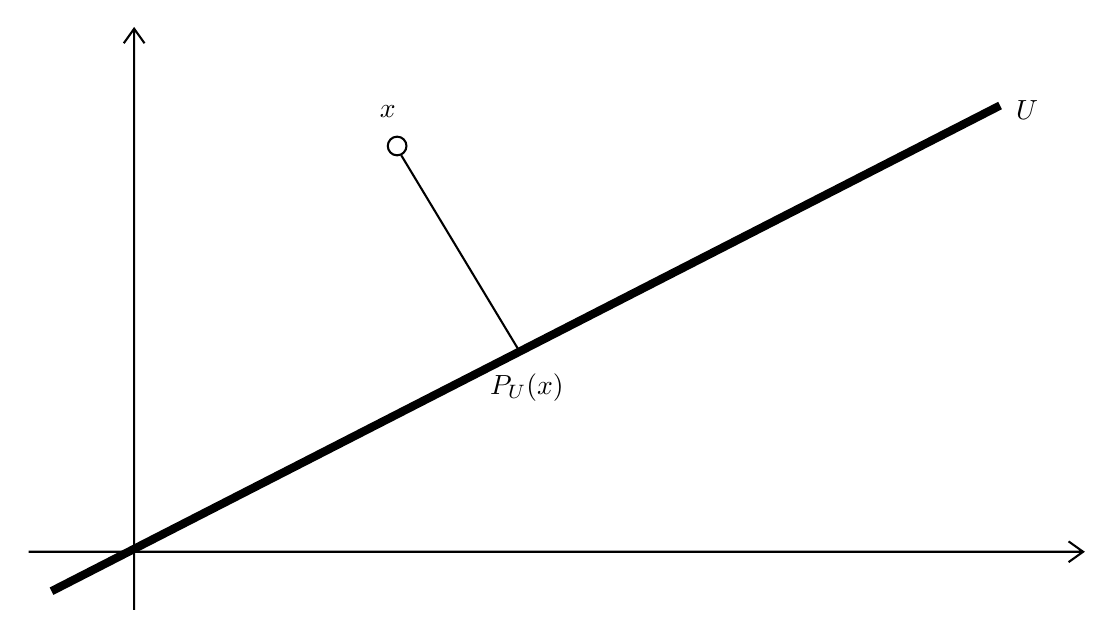
\begin{tikzpicture}[x=0.75pt,y=0.75pt,yscale=-1,xscale=1]
%uncomment if require: \path (0,300); %set diagram left start at 0, and has height of 300

%Shape: Axis 2D [id:dp7098119764904821] 
\draw  (50,256.93) -- (558,256.93)(100.8,4.93) -- (100.8,284.93) (551,251.93) -- (558,256.93) -- (551,261.93) (95.8,11.93) -- (100.8,4.93) -- (105.8,11.93)  ;
%Straight Lines [id:da9071558730776327] 
\draw [line width=3]    (61,275.93) -- (518,41.93) ;


%Straight Lines [id:da7398348018165936] 
\draw    (210,68.93) ;


%Shape: Circle [id:dp7764692603132283] 
\draw   (223,61.43) .. controls (223,58.95) and (225.01,56.93) .. (227.5,56.93) .. controls (229.99,56.93) and (232,58.95) .. (232,61.43) .. controls (232,63.92) and (229.99,65.93) .. (227.5,65.93) .. controls (225.01,65.93) and (223,63.92) .. (223,61.43) -- cycle ;
%Straight Lines [id:da721943207149605] 
\draw    (229.5,65.93) -- (286.5,160.43) ;



% Text Node
\draw (531,43.93) node  [align=left] {$U$};
% Text Node
\draw (223,44.93) node  [align=left] {$x$};
% Text Node
\draw (290,177.93) node  [align=left] {$P_U(x)$};


\end{tikzpicture}

		\caption{Skizze zur Bestapproximation}
		\label{Abb:Bestapproximation}
	\end{center}
\end{figure}

\begin{proof}
	\betone{Zeige \ref{item:satz2.10(1)}:}\\
	Sei $u\in U$ beliebig.
	Dann folgt aus der Definition der Projektion:
	\begin{align*}
		x&=P_U(x)+v\qquad\exists v\in U^\perp\\
		\implies\norm{x-u}^2&=\norm[\Big]{\big(\underbrace{P_U(x)-u}_{\in U}\big) +v}^2
		\overset{\ref{satz2.1}\ref{item:satz2.1(1)}}{=}
		\underbrace{\norm{P_U(x)-u}^2}_{\geq0}+\norm{v}^2
		\geq\norm{v}^2=\norm{x-P_U(x)}^2
	\end{align*}
	Und Gleichheit gilt genau dann, wenn $u=P_U(x)$.\nl
	\betone{Zeige \ref{item:satz2.10(2)}:}
	\begin{align*}
		x&=P_U(x)+P_{U^\perp}(x)\\
		&\implies x-P_U(x)=P_{U^\perp}(x)\\
		&\implies x-P_U(x)\in U^\perp
	\end{align*}
	\betone{Zeige \ref{item:satz2.10(3)}:}
	\begin{align*}
		x-u\in U^\perp
		\implies x=\underbrace{u}_{\in U}+\underbrace{(x-u)}_{\in U^\perp}
		\implies u=P_U(x)
	\end{align*}
\end{proof}

\begin{satz}\label{satz:2.11}
	Sei
	\begin{align*}
		A=\big(a_1,\ldots,a_n\big)=\begin{pmatrix}
			b_1'\\
			\vdots\\
			b_m'
		\end{pmatrix}\in M(m\times n)
	\end{align*}
	d.h. $a_i\in\R^m$ ist $i$-te Spalte von $A$ bzw. $b_i\in\R^n$ und $b_i'=i$-te Zeile von $A$.
	Dann gilt:
	\begin{enumerate}[label=(\alph*)]
		\item $\begin{aligned}
			 \dim\Big(\spann\big(a_1,\ldots,a_n\big)\Big)
			 =\dim\Big(\spann\big(b_1,\ldots,b_m\big)\Big) 
			 \label{item:satz2.11(a)}
		\end{aligned}$\\
		Der gemeinsame Wert $\Rg(A)$ heißt \define{Rang} von $A$.
		\index{Rang}  
		\item $\begin{aligned}
			 \Rg(A)=\Rg(A')=
			 \label{item:satz2.11(b)}
		\end{aligned}$ maximale Anzahl linear unabhängiger Zeilen / Spalten von $A$
		\item $\begin{aligned}
			\Rg(A)\leq\min\set{m,n}
			\label{item:satz2.11(c)}
		\end{aligned}$
		\item $\begin{aligned}
			B\in M(n\times p)\implies\left\lbrace
			\begin{array}{l}
				\Rg(A\mal B)\leq\min\set{\Rg(A),\Rg(B)}\\
				\Rg(A\mal B)\geq\Rg(A)+\Rg(B)-n
			\end{array}\right.
			\label{item:satz2.11(d)}
		\end{aligned}$
		\item Seien $S\in M(m\times m),~T\in M(n\times n)$ invertierbar.
		Dann gilt: \label{item:satz2.11(e)}
		\begin{align*}
			\rg(S\mal A\mal T)=\Rg(A)
		\end{align*}
	\end{enumerate}
\end{satz}

\begin{proof}
	Siehe Koecher \cite{koecher2013lineare}, Seite 57 ff.
\end{proof}

\begin{satz}[Dimensionsformel]\label{satz:2.12Dimensionsformel}\enter
	Sei $A\in M(m\times n)$. Setze
	\index{Bild einer Matrix}\index{Kern einer Matrix}\index{Dimensionsformel}
	\begin{align*}
		\Kern(A):=\set{x\in\R^n:A\mal x=0}\qquad
		\Bild(A):=\set{A\mal x:x\in\R^n}
	\end{align*}
	Dann gilt:
	\begin{align*}
		\dim\big(\Kern(A)\big)+\dim\big(\Bild(A)\big)=n
	\end{align*}
\end{satz}

\begin{proof}
	Siehe Koecher \cite{koecher2013lineare}, Seite 39 ff.
\end{proof}

\begin{satz}\label{satz:2.13}
	Sei $A\in M(m\times n)$ mit $m\geq n$.
	Dann gilt: \index{Vollrang}
	\begin{align*}
		A'\mal A\text{ invertierbar}\iff\Rg(A)=n\iff: A\text{ hat \define{Vollrang}}
	\end{align*}
\end{satz}

\begin{proof}
	\betone{Zeige "$\Longrightarrow$":}
	\begin{align*}
		n&=\Rg(I_n)
		=\Rg\klammern{A'\mal A\mal(A'\mal A)^{-1}}
		\overset{\text{\ref{satz:2.11}\ref{item:satz2.11(e)}}}{=}
		\rg(A'\mal A)
		\overset{\text{\ref{satz:2.11}\ref{item:satz2.11(d)}+\ref{satz:2.11}\ref{item:satz2.11(b)}}}{\leq}
		\Rg(A)
		\leq n
	\end{align*}
	\betone{Zeige "$\Longleftarrow$":} Es gilt:
	\begin{align*}
		\Bild(A)=\spann\big(a_1,\ldots,a_n\big)
	\end{align*}
	wobei $a_i:=A\mal e_i$ die $i$-te Spalte von $A$ ist, denn:
	\begin{align}
		A\mal x \nonumber
		&=A\klammern{\sum\limits_{i=1}^n x_i\mal e_i}
		=\sum\limits_{i=1}^n x_i\mal A\mal e_i
		=\sum\limits_{i=1}^n x_i\mal A_i
		\qquad\forall x=\big(x_1,\ldots,x_n\big)'\in\R^n\\
		\overset{\ref{satz:2.12Dimensionsformel}}&{\implies}\nonumber
		\dim\big(\Kern(A)\big)=0\\
		&\implies \Kern(A)=\set{0}\label{eq:ProofSatz2.13Stern}\tag{$*$}\\
		&\implies\Kern(A'\mal A)=\set{0}, \label{eq:ProofSatz2.13SternStern}\tag{$**$}
	\end{align}
	denn:
	\begin{align*}
		A'\mal A=0
		&\implies (x'\mal A')\mal A\mal x=(A\mal x)'\mal A\mal x=\norm{A\mal x}^2
		\implies\norm{A\mal x}=0\\
		&\implies A\mal x=0\implies x\in\Kern(A)
		\overset{\eqref{eq:ProofSatz2.13Stern}}{\implies}x=0
	\end{align*}
	Aus \eqref{eq:ProofSatz2.13SternStern} folgt, dass $A'\mal A$ injektiv ist.
	Gemäß Satz \ref{satz:2.12Dimensionsformel} ist $A'\mal A$ auch surjektiv, also insgesamt bijektiv.
	Also ist $A'\mal A$ invertierbar.
\end{proof}

\begin{satz}\label{satz2.14}
	Sei $A\in M(m\times n),~B\in M(n\times m)$.
	Dann gilt: \index{Spur einer Matrix}
	\begin{align*}
		\Spur(A\mal B)=\Spur(B\mal A)
		\qquad\mit\qquad
		\Spur(A):=\sum\limits_{i=1}^n a_{i,i}
	\end{align*}
	(Die Spur einer Matrix ist die Summe der Diagonalelemente.)
\end{satz}

\begin{proof}
	\begin{align*}
		\Spur(A\mal B)
		\overset{\Def}&{=}
		\sum\limits_{i=1}^m(A\mal B)_{i,i}\\
		&=\sum\limits_{i=1}^m\klammern{\sum\limits_{j=1}^n(A)_{i,j}\mal(B)_{j,i}}\\
		&=\sum\limits_{j=1}^n\sum\limits_{i=1}^m (B)_{j,i}\mal(A)_{i,j}\\
		&=\sum\limits_{j=1}^n(B\mal A)_{j,j}\\
		&=\Spur(B\mal A)
	\end{align*}
\end{proof}

\begin{erinnerung}\
	\begin{enumerate}
		\item $A=\big(a_1,\ldots,a_n\big)\in M(n\times n)$ heißt \define{orthonormal / orthogonal}
		\begin{align*}
			:&\iff\forall i,j\in\set{1,\ldots,n}:\scaProd{a_i}{a_j}=\delta_{i,j}\\
			&\iff A^T=A^{-1}
		\end{align*}
		\item Sei $A\in M(n\times n)$. 
		Dann heißt $\lambda\in\C$ \define{Eigenwert (EW)} von $A$ \index{Eigenwert}\index{Eigenvektor}
		\begin{align*}
			:\iff\exists x\in\R^n\setminus\set{0}:A\mal x=\lambda\mal x
		\end{align*}		 
		In diesem Fall heißt $x$ der zum Eigenwert $\lambda$ gehörende \define{Eigenvektor (EV)} von $A$.
	\end{enumerate}
\end{erinnerung}

\begin{satz}\label{satz:2.15}
	Sei $A\in M(n\times n)$ symmetrisch.
	Dann existiert eine orthogonale / orthonormale Matrix
	$B=\big(v_1,\ldots,v_n\big)$ bestehend aus Eigenvektoren (EV) von $A$ mit
	\begin{align*}
		B'\mal A\mal B=\begin{pmatrix}
			\lambda_1 & 0 & 0\\
			0 & \ddots & 0\\
			0 & 0 & \lambda_n
		\end{pmatrix}=:D=:\Diag\big(\lambda_1,\ldots,\lambda_n\big)
	\end{align*}
	Dabei ist $\lambda_i\in\R$ Eigenwert (EW) von $A$ zum Eigenwert $v_i$ ($i\in\set{1,\ldots,n}$).
\end{satz}

\begin{proof}
	\betone{Teil 1:} Siehe Koecher \cite{koecher2013lineare} Seite 194.\nl
	\betone{Teil 2:} Zunächst gilt $B'\mal B=I_n$, denn
	\begin{align*}
		\scaProd{v_i}{v_j}=v_i'\mal v_j=\delta_{i,j}=\left\lbrace\begin{array}{cl}
			0,&\falls i\neq j\\
			1,&\falls i=j
		\end{array}\right.
	\end{align*}
	Also ist $B'$ Linksinverses von $B$ und damit auch Rechtsinverses.
	\begin{align*}
		A\mal v_i
		&=B\mal D\mal\underbrace{B'\mal v_i}_{=e_i}
		=B\mal D\mal e_i
		=B\mal\lambda_i\lambda e_i
		=\lambda_i\mal B\mal e_i
		=\lambda_i\lambda\mal v_i
	\end{align*}
	Dass die Eigenwerte hierbei reellwertig sind, folgt aus der Symmetrie.
\end{proof}

\begin{satz}\label{satz:2.16}
	Sei $A$ symmetrisch und \define{idempotent}, d.h. $A^2=A$.
	Dann gilt: \index{idempotente Matrix}
	\begin{align*}
		\Rg(A)=\Spur(A)
	\end{align*}
\end{satz}

\begin{proof}
	Für $\lambda_1,\ldots,\lambda_d$ in Satz \ref{satz:2.15} gilt o.B.d.A. (sonst $v_i$'s vertauschen) $\lambda_1\geq\lambda_2\geq\ldots\geq\lambda_n$.\\
	Sei $x$ Eigenvektor von $A$ zum Eigenwert $\lambda$.
	Dann gilt:
	\begin{align*}
		\lambda\mal x=A\mal x=A(A\mal x)=A\mal\lambda\mal x=\lambda\mal A\mal x=\lambda^2\mal	x\\
		\overset{x\neq0}{\implies}
		\lambda=\lambda^2\in\R\implies \lambda\in\set{0,1}
	\end{align*}
	Gemäß Satz \ref{satz:2.15} existiert eine orthogonale Matrix $B$ derart, dass
	\begin{align}\label{eq:ProofSatz2.16Star}\tag{$*$}
		B'\mal A\mal B&=\begin{pmatrix}
			1 & 0 &\hdots & \hdots & \hdots & 0\\
			0 & \ddots & \ddots & \ddots & \ddots & \vdots\\
			\vdots & \ddots & 1 & \ddots & \ddots & \vdots\\
			\vdots & \ddots & \ddots & 0 & \ddots & \vdots\\
			\vdots & \ddots & \ddots & \ddots &  \ddots & \vdots\\
			0 & \hdots & \hdots & \hdots & \hdots & 0
		\end{pmatrix}=:D\\ \nonumber
		\implies\Rg(A)
		\overset{\text{\ref{satz:2.11}\ref{item:satz2.11(e)}}}&{=}
		\rg(B'\mal A\mal B)\\ \nonumber
		\overset{\eqref{eq:ProofSatz2.16Star}}&{=}
		\Rg(D)\\\nonumber
		\overset{\text{\ref{satz:2.11}\ref{item:satz2.11(a)}}}&{=}
		\Spur(D)\\\nonumber
		\overset{\eqref{eq:ProofSatz2.16Star}}&{=}
		\Spur\big(B'\mal(A\mal B)\big)\\\nonumber
		\overset{\ref{satz2.14}}&{=}
		\Spur\big(A\mal\underbrace{(B\mal B')}_{=I_n}\big)\\\nonumber
		&=\Spur(A)
	\end{align}
\end{proof}

\begin{satz}\label{satz2.17}
	Sei $A\in M(m\times n)$. Dann gilt:
	\begin{align*}
		\Kern(A)&=\big(\Bild(A')\big)^\perp\\
		\overset{\text{\ref{satz2.1}\ref{item:satz2.1(3)}\ref{item:satz2.1(3ii)}}}{\iff}
		\Kern(A)^\perp&=\Bild(A')
	\end{align*}
\end{satz}

\begin{proof}
	Sei $x\in\Kern(A)$.
	\begin{align*}
		&x\in\Kern(A)\\
		&\iff A\mal x=0\\
		&\iff\scaProd{b_i}{x}=0 &&\forall i\in\set{1,\ldots,n}\text{wobei $b_i':=i$-te Zeile von $A$}\\
		&\iff\scaProd{y}{x}=0 &&\forall y\in\spann\big(b_1,\ldots,b_m\big)\\
		&\iff x\perp\spann\big(b_1,\ldots,b_m\big)
		\overset{\text{vgl.\ref{satz:2.13}}}{=}		
		\Bild(A)\\
		&\iff x\in\Bild(A')^\perp
	\end{align*}
	denn:
	\begin{align*}
		\scaProd{\sum\limits_{i=1}^m \alpha_i\mal b_i}{x}=\sum\limits_{i=1}^m\underbrace{\scaProd{b_i}{x}}_{=0~\forall i}=0
	\end{align*}
\end{proof}

\begin{satz}\label{satz:2.18}
	Seien $U_1,U_2\subseteq\R^n$ Untervektorräume des $\R^n$.
	Dann gilt
	\begin{enumerate}[label=(\arabic*)]
		\item $\begin{aligned}
			\big(U_1+U_2\big)^\perp=U_1^\perp\cap U_2^\perp
			\label{item:satz2.18(1)}
		\end{aligned}$
		\item $\begin{aligned}
			\big(U_1\cap U_2\big)^\perp=U_1^\perp+ U_2^\perp
			\label{item:satz2.18(2)}
		\end{aligned}$
	\end{enumerate}
\end{satz}

\begin{proof}
	\betone{Zu \ref{item:satz2.18(1)} zeige "$\subseteq$":}
	\begin{align*}
		U_1+U_2\overset{0\in U_1\cap U_2}{\supseteq} U_i\qquad\forall i\in\set{1,2}\\
		\implies \big(U_1+U_2\big)^\perp\subseteq U_i^\perp
		\implies\big(U_1+U_2)^\perp\subseteq U_1^\perp\cap U_2^\perp
	\end{align*}
	\betone{Zu \ref{item:satz2.18(1)} zeige "$\supseteq$":}\\
	Sei $x\in U_1^\perp\cap U_2^\perp$.
	Sei $y\in U_1+U_2$.	
	Dann gilt:
	\begin{align*}
		\exists u_1\in U_1,u_2\in U_2: y=u_1+u_2\\
		\implies\scaProd{x}{y}\overset{\Lin}{=}\underbrace{\scaProd{x}{u_1}}_{
			\overset{x\in U_1^\perp}{=}0		
		}+\underbrace{\scaProd{x}{u_2}}_{
			\overset{x\in U_2^\perp}{=}0
		}
		\implies x\perp U_1+U_2
		\implies x\in\big(U_1+U_2\big)^\perp
	\end{align*}
	\betone{Zeige \ref{item:satz2.18(2)}:}\\
	Wende \ref{item:satz2.18(1)} auf $U_1^\perp$ und $U_2^\perp$ an:
		\begin{align*}
		\big(U_1\cap U_2\big)^\perp
		\overset{\ref{satz2.1}}&{=}
		\Big(\big(U_1^\perp\big)^\perp\cap\big(U_2^\perp\big)^\perp\Big)^\perp
		\overset{\ref{item:satz2.18(1)}}{=}
		\Big(\big(U_1^\perp+U_2^\perp\big)^\perp\Big)^\perp
		\overset{\ref{satz2.1}}{=}
		U_1^\perp+U_2^\perp
	\end{align*}		
\end{proof}

\begin{satz}\label{satz2.19}
	Sei $A\in M(m\times n)$, $U\subseteq\R^n$ Untervektorraum von $\R^n$.
	Dann gilt:
	\begin{align*}
		\big(\Kern(A)\cap U\big)^\perp
		=\Bild\big(P_U A'\big)
	\end{align*}
\end{satz}

\begin{proof}
	\betone{Zeige "$\subseteq$":}
	\begin{align*}
		\big(\Kern(A)\cap U\big)^\perp
		\overset{\ref{satz:2.18}\ref{item:satz2.18(2)}}&{=}
		\big(\Kern(A)^\perp+U^\perp\big)\cap U
		\overset{\ref{satz2.17}}{=}
		\big(\Bild(A')+U^\perp\big)\cap U
	\end{align*}
	Sei nun $x\in\big(\Bild(A')+U^\perp\big)\cap U$.
	Dann: $\exists y\in\R^m,\exists v\in U^\perp$ mit
	\begin{align}\label{eq:Proof2.19Stern}\tag{$*$}
		x=A'\mal y+v
		\overset{\ref{satz2.5}}{=}
		A'\mal y+P_{U^\perp} v
		\overset{\ref{satz2.9}}{=}
		A'\mal y+\big(I_n-P_U\big)\mal v\\ \nonumber
		\implies x
		\overset{\ref{satz2.5},x\in U}{=}
		P_U x
		\overset{\eqref{eq:Proof2.19Stern}}{=}
		P_U A'\mal y+\underbrace{P_U\big(I_n-P_u\big)}_{=P_U-P_U^2\overset{\ref{satz2.7}}{=}0}\mal v
		=\big(P_U A'\big)\mal y\in\Bild\big(P_U A'\big)
	\end{align}		
	
	\betone{Zeige "$\supseteq$":}\\
	Sei $x\in\Bild\big(P_U A'\big)$.
	Dann gilt
	\begin{align*}
		x=P_U A'\mal y\qquad\exists y\in\R^m
	\end{align*}
	und somit $x\in U$.
	Ferner sei $z\in\Kern(A)\cap U$. Folglich:
	\begin{align*}
		\scaProd{x}{z}=x'\mal z
		=y'\mal(A')'\mal P_U' z
		\overset{\ref{satz2.8}}{=}
		y'\mal A\mal P_U z
		\overset{z\in U,\ref{satz2.5}}{=}
		y'\mal (A\mal z)
		\overset{z\in\Kern(A)}{=}
		y'\mal 0
		=0
	\end{align*}
	Also ist $\scaProd{x}{z}=0$ für alle $z\in\Kern(A)\cap U$.
	Somit ist $x\in\big(\Kern(A)\cap U\big)^\perp$.
\end{proof}

\begin{satz}\label{satz2.20}
	Seien $U_1\subseteq U_2\subseteq\R^n$ Untervektorräume.
	Dann gilt:
	\begin{align*}
		P_{U_1}\mal P_{U_2}=P_{U_2}\mal P_{U_1}=P_{U_1}
	\end{align*}
\end{satz}

\begin{proof}
	\begin{align*}
		P_{U_2}\underbrace{\big(P_{U_1} x\big)}_{\in U_1\subseteq U_2}
		\overset{P_{U_1}x\in U_2,\ref{satz2.5}}{=}
		P_{U_1}x\qquad\forall x\in\R^n
	\end{align*}
	Ferner sei $x\in\R^n$. 
	Dann ist $x=u_1+v_1=u_2+v_2$ mit $u_i\in U_i$ und $v_i\in U_i^\perp$, $i\in\set{1,2}$.
	Sowie
	\begin{align}\label{eq:Proof2.20Stern}\tag{$*$}
		U_2^\perp\subseteq U_1^\perp
	\end{align}		
	Damit:
	\begin{align*}
		P_{U_1}P_{U_2}(x)
		&=P_{U_1}\big(P_{U_2}(x)\big)\\
		&=P_{U_1}(u_2)\\
		\overset{\ref{satz2.9}}&{=}
		\big(\id-P_{U_1^\perp}\big)(u_2)\\
		&=u_2-P_{U_1^\perp}(\underbrace{u_2}_{=x-v_2})\\
		\overset{\Lin}&{=}
		u_2-P_{U_1^\perp}(x)+\underbrace{P_{U_1^\perp}(\underbrace{v_2}_{
			\overset{\eqref{eq:Proof2.20Stern}}{=}u_1^\perp		
		})}_{=v_2}\\
		&=x-P_{U_1^\perp}(x)\\
		&=\big(\id-P_{U_1^\perp}\big)(x)\\
		\overset{\ref{satz2.9}}&{=}
		P_{U_1}(x)\\
		\implies P_{U_1}P_{U_2}=P_{U_1}
	\end{align*}
\end{proof}

\begin{satz}\label{satz2.21}
	Sei $U_1\subseteq U_2\subseteq\R^n$ Untervektorräume.
	Dann gilt:
	\begin{align*}
		P_{U_2}=P_{U_1}+P_{U_1^\perp\cap U_2}
	\end{align*}
\end{satz}

\begin{proof}
	Sei zunächst $x\in U_2$.
	Es gilt wegen Satz \ref{satz2.3}:
	\begin{align*}
		x=u+v\qquad\exists u\in U_1,v\in U_1^\perp
	\end{align*}
	Insbesondere:
	\begin{align*}
		u=P_{U_1}(x),\qquad v=P_{U_1^\perp}(x)
	\end{align*}
	Da $x\in U_2$ und $u\in U_2$ (wegen $U_1\subseteq U_2$) folgt $v=x-u\in U_2$.
	Also $v\in U_1^\perp\cap U_2$. Es folgt:
	\begin{align*}
		v\overset{\ref{satz2.5}}{=}
		P_{U_1^\perp\cap U_2}(v)
		=P_{U_1^\perp\cap U_2}\big(P_{U_1^\perp}(x)\big)
		\overset{\ref{satz2.20}}{=}
		P_{U_1^\perp\cap U_2}(x)
	\end{align*}
	Somit:
	\begin{align}\label{eq:Proof2.21Stern}\tag{$*$}
		P_{U_2}(x)
		\overset{x\in U_2,\ref{satz2.5}}{=}
		x
		=u+v
		=P_{U_1}(x)+P_{U_1^\perp\cap U_2}(x)
		\qquad\forall x\in U_2
	\end{align}
	Sei jetzt $x\in\R^n$ beliebig.
	Dann folgt:
	\begin{align*}
		P_{U_2}(x)
		\overset{\ref{satz2.7}}{=}
		P_{U_2}\big(\underbrace{P_{U_2}(x)}_{\in U_2}\big)
		\overset{\eqref{eq:Proof2.21Stern}}{=}
		P_{U_1}\big(P_{U_2}(x)\big)+P_{U_1^\perp\cap U_2}\big(P_{U_2}(x)\big)
		\overset{\ref{satz2.20}}{=}
		P_{U_1}(x)+P_{U_1^\perp\cap U_2}(x)
	\end{align*}
\end{proof}

Der folgende Satz hilft uns, die Existenz des Schätzers sicherzustellen und gibt uns eine Möglichkeit, diesen auszurechnen.

\begin{notation}
	\begin{align*}
		\argmin\limits_{y\in\R^p} f(y):=\set{z\in\R^p:f(z)\leq f(y)~\forall y\in\R^p}
	\end{align*}
\end{notation}

\begin{satz}\label{satz2.22}
	Sei $A\in M(n\times p)$ mit $n\geq p$ und $x\in\R^n$ fest.
	Dann gilt:
	\begin{enumerate}[label=(\alph*)]
		\item Die Minimalstelle \label{item:satz2.22(a)}
		\begin{align*}
			y_0\in\argmin\limits_{y\in\R^p}\norm{x-A\mal y}
			=\argmin\limits\set[\big]{\norm{x-A\mal y}:y\in\R^p}
		\end{align*}
		existiert und erfüllt die \define{Normalgleichung} \index{Normalgleichung}
		\begin{align*}
			A'\mal A\mal y_0=A'\mal x.
		\end{align*}
		Umgekehrt ist jede Lösung der Normalgleichung eine Minimalstelle
		\begin{align*}
			\argmin\limits_{y\in\R^p}\norm{y-A\mal x}.
		\end{align*}
		Ferner gilt:
		\begin{align*}
			A\mal y_0=P_{\Bild(A)}(x)
		\end{align*}
		\item Falls $\Rg(A)=p$ (also Vollrang), so gilt \label{item:satz2.22(b)}
		\begin{align*}
			y_0=\big(A'\mal A\big)^{-1}\mal A'\mal x
			\qquad\und\qquad
			P_{\Bild(A)}=A\mal\big(A'\mal A\big)^{-1}\mal A'
		\end{align*}
	\end{enumerate}
\end{satz}

\begin{proof}
	\betone{Zeige \ref{item:satz2.22(a)}:}\\
	$U:=\Bild(A)$ ist Untervektorraum des $\R^n$.
	Nach Satz \ref{satz2.10}\ref{item:satz2.10(1)} ist $u_0:=P_U(x)$ eine eindeutige Minimalstelle von
	\begin{align*}
		\set[\big]{\norm{x-u}:u\in U}=\set[\big]{\norm{x-A\mal y}:y \in\R^p}
	\end{align*}
	Da $u_0\in\Bild(A)$, ist
	\begin{align*}
		M:=A^{-1}\big(\set*{u_0}\big)=\set{y\in\R^p:A\mal y=u_0}
		\neq\emptyset
	\end{align*}
	und für alle $y_0\in M$ gilt:
	\begin{align*}
		\norm{x-A\mal y_0}=\norm{x-u_0}
		\leq\norm{x-A\mal y}\qquad\forall y\in\R^p
	\end{align*}
	d.h. $y_0$ ist Minimalstelle und wegen $y_0\in M$ gilt:
	\begin{align}\label{eq:Proof2.22Stern}\tag{$*$}
		A\mal y_0&=u_0=P_{\Bild(A)}(x)
	\end{align}
	Mit Satz \ref{satz2.10}\ref{item:satz2.10(2)} folgt:
	\begin{align*}
		&\hspace{10mm}x-A\mal y_0\perp A\mal y\qquad\forall y\in\R^p\\
		&\iff &0&=\scaProd{x-A\mal y_0}{A\mal y}\\
		&&\overset{\text{Sym}}&{=}
		\scaProd{A\mal y}{x-A\mal y_0}\\
		&&&=(A\mal y)'\mal(x-A\mal y_0)\\
		&&&=y'\mal A'\mal(x-A\mal y_0)\\
		&&&=y'\mal(A'\mal x-A'\mal A\mal y_0)\\
		&&&=\scaProd{y}{A'\mal x-A'\mal A\mal y_0}\qquad\forall y\in\R^p\\
		&\iff A'\mal x-A'\mal A\mal y_0\perp\R^d\\
		&\iff A'\mal x-A'\mal A\mal y_0=0\\
		&\iff A'\mal A\mal y_0=A'\mal x
	\end{align*}
	Hierbei geht ein:
	\begin{align*}
		z\perp\R^p\iff\scaProd{z}{y}=0~\forall y\in\R^p\\
		\overset{y=z}{\implies}\scaProd{z}{z}=0
		\implies z=0\\
		z=0\implies\scaProd{z}{y}=0~\forall y\in\R^p
	\end{align*}
	Umgekehrt ist jede Lösung $y_0$ Der Normalgleichung Minimalstellen von 
	\begin{align*}
		y\mapsto\norm{x-A\mal y},
	\end{align*}
	denn:
	\begin{align*}
		A'\mal A\mal y_0=A'\mal x
		\overset{\text{s.o.}}&{\iff}
		x-\underbrace{A\mal y_0}_{\in\Bild(A)}\perp\Bild(A)\\
		\overset{\ref{satz2.10}\ref{item:satz2.10(3)}}&{\implies}
		A\mal y_0=P_{\Bild(A)}(x)=u_0\\
		&\implies y_0\text{ ist Minimalstelle}
	\end{align*}
	
	\betone{Zeige \ref{item:satz2.22(b)}:}\\
	Gelte also $\Rg(A)=p$.
	Dann folgt aus Satz \ref{satz:2.13}, dass $A'\mal A$ invertierbar ist.
	Aus \ref{item:satz2.22(a)} folgt dann
	\begin{align*}
		y_0&=\big(A'\mal A\big)^{-1}\mal A'\mal x\\
		\overset{\eqref{eq:Proof2.22Stern}}{\implies}
		P_{\Bild(A)}(x)=A\mal(A'\mal A)^{-1}\mal A'\mal x\qquad\forall x\in\R^n
	\end{align*}
\end{proof}

\begin{definition}\label{def2.23}
	$A\in M(n\times n)$ symmerisch heißt
	\begin{enumerate}
		\item \define{positiv definit}
		\index{positiv definit}
		\begin{align*}
			\defiff\forall x\in\R^n\setminus\set{0}:x'\mal A\mal x>0
		\end{align*}
		\item \define{nichtnegativ definit}
		\index{nichtnegativ definit}
		\begin{align*}
			\defiff\forall x\in\R^n\setminus\set{0}:x'\mal A\mal x\geq0
		\end{align*}
	\end{enumerate}			
\end{definition}

\begin{satz}\label{satz2.24}
	Sei $A\in M(n\times n)$ positiv definit.
	Dann gilt:
	\begin{enumerate}[label=(\alph*)]
		\item Alle Eigenwerte von $A$ sind positiv.
		\label{item:satz2.24(a)}
		\item Es existiert $R\in M(n\times n)$ positiv definit mit $A=R^2$.
		Bezeichnung: $A^{\frac{1}{2}}:=R$
		\label{item:satz2.24(b)}
		\item $A$ ist invertierbar und $A^{-1}$ ist positiv definit.
		\label{item:satz2.24(c)}
	\end{enumerate}
\end{satz}

\begin{proof}
	\betone{Zeige \ref{item:satz2.24(a)}:}\\
	Sei $\lambda$ Eigenwert zum Eigenvektor $x\neq0$.
	Dann gilt $A\mal x=\lambda\mal x$ nach Definition des Eigenwertes.
	\begin{align*}
		0
		\overset{A\text{ p.d.}}&{<}
		x'\mal A\mal x
		=x'\mal\lambda\mal x
		=\lambda\mal\norm{x}^2
		\overset{\norm{x}>0}{\implies}
		\lambda>0
	\end{align*}
	
	\betone{Zeige \ref{item:satz2.24(b)}:}\\
	Gemäß Satz \ref{satz:2.15} existiert eine orthogonale Matrix $B\in M(n\times n)$ mit
	\begin{align*}
		A=B\mal D\mal B',\qquad D:=\diag\big(\lambda_1,\ldots,\lambda_n\big)
	\end{align*}
	wobei $\lambda_1,\ldots,\lambda_n$ Eigenwerte von $A$ sind, die wegen \ref{item:satz2.24(a)} alle positiv sind.
	Setze
	\begin{align*}
		R:=B\mal\sqrt{D}\mal B',\qquad\sqrt{D}:=\diag\klammern{\sqrt{\lambda_1},\ldots,\sqrt{\lambda_n}}\\
		\implies
		R^2=B\mal \sqrt{D}\mal\underbrace{B'\mal B}_{=I_n}\mal \sqrt{D}\mal B'
		=B\mal\sqrt{D}\mal\sqrt{D}\mal B'
		=B\mal D\mal B'
		=A
	\end{align*}
	Ferner ist $R$ symmetrisch, denn 
	\begin{align*}
		R'\overset{\Def}{=}\big(B\mal\sqrt{D}\mal B'\big)'=B''\mal\sqrt{D}'\mal B'
		\overset{D~\diag}{=}B\mal\sqrt{D}\mal B'
	\end{align*}
	Weiterhin gilt für alle $x\neq0$:
	\begin{align*}
		x'\mal R\mal x
		\overset{\Def}&{=}
		x'\mal B\mal\sqrt{D}\mal\underbrace{B'\mal x}_{=:y}
		=y'\mal\sqrt{D}\mal y=\sum\limits_{i=1}^n\underbrace{\sqrt{\lambda_i}}_{>0}\mal y_i^2
		>0
	\end{align*}
	und $y\neq 0$, da $x\neq0$ und $\Kern(B')=\set{0}$ (weil $B'$ invertierbar).\nl
	\betone{Zeige \ref{item:satz2.24(c)}:}\\
	$A=R\mal R$ und $\R$ ist invertierbar, da $B$, $\sqrt{D}$ und $B'$ invertierbar sind.
	Somit ist auch $A$ invertierbar.
	\begin{align*}
		A^{-1}=R^{-1}\mal R^{-1}=S\mal S
		\qquad\mit\qquad S:=R^{-1}\text{ invertierbar und symmetrisch}\\
		\implies x'\mal A^{-1}\mal x=x'\mal S'\mal S\mal x=\scaProd{S\mal x}{S\mal x}=\norm{S\mal x}^2>0,
	\end{align*}
	da $x\neq0$ und $\Kern(S)=\set{0}$.\\
	($S$ ist symmetrisch wegen $S'=(R^{-1})'=(R')^{-1}=R^{-1}=S$.)
\end{proof}

\begin{bemerkung} %ohne Nummer
	Falls $A$ in Satz \ref{satz2.24} nichtnegativ definit ist (statt positiv definit), so gelten \ref{item:satz2.24(a)} und \ref{item:satz2.24(b)} analog mit "nichtnegativ" anstelle von "positiv".
	Dies zeigt der Beweis von \ref{item:satz2.24(a)} und \ref{item:satz2.24(b)}.
\end{bemerkung}
